\section{Remnants with a history: accumulation, halos and cosmic time}\label{sec:remnant}

Section~\ref{sec:sparc} tested the stochastic remnant of Section~\ref{sec:darkmatter} as Oppenheim and Russo derived it~\cite{oppenheimrusso},
a static, constant extra acceleration $|\gamma_1|/2$, and rejected it: at low acceleration the excess $g_{\rm obs}-g_{\rm bar}$ over the
Newtonian acceleration of the baryons rises with $g_{\rm bar}$ with logarithmic slope 0.44, where a constant gives 0 \chk{sparc:S2d}. GUID's
cosmology (Section~\ref{sec:cosmo}) is a long evolution, and Hypothesis~H7 keeps the remnants of interactions in the frame, so they may
accumulate. Here we test what the theory allows once that history is included: an accumulated stochastic term, its dependence on each
galaxy's history, the contained remnant (primordial black holes, which form cold dark matter halos), the two together, the change of scale
with cosmic time, and what cannot be fitted at all. The result: an accumulated term of the self-consistent form fits the rotation curves as
well as the radial acceleration relation (RAR), but it is MOND's phenomenology, fails the solar system, carries no galaxy-specific history and
has the wrong arrow in time; once cold halos are present, the data leave it at most a few per cent of the dark acceleration. The two remnants
compete rather than combine.

Data, cuts, error model and the likelihoods L1 (full error model) and L2 (velocity errors and a fitted floor) are those of
Section~\ref{sec:sparc}: $N=2696$ points in 147 SPARC galaxies~\cite{lelli2016}, with $\Upsilon_{\rm disk}=0.5$ and $\Upsilon_{\rm bulge}=0.7$.
The script imports that pipeline and reproduces its universal fits to $10^{-4}$. Uncertainties come from resampling galaxies (1000 draws),
because points within a galaxy share distance, inclination and $\Upsilon$ errors and the point-wise BIC, $-2\ln L+k\ln N$, overstates the
evidence.

\subsection{The accumulated stochastic remnant}\label{sec:remnant-acc}

\paragraph{The accumulation hypothesis.} \tagH\ The random kicks that the frame's diffusion leaves in the field (Section~\ref{sec:cq})
accumulate over cosmic time as a random walk. If the variance of the extra acceleration grows with the local source and with time,
$\langle\delta g^2\rangle=\kappa\,g_{\rm bar}\,t$, and the entropic attraction is of the order of its root mean square, the extra acceleration
is the geometric mean of $g_{\rm bar}$ and an accumulated scale $a_{\rm acc}\equiv\kappa t$. This is a hypothesis; the classical-quantum
dynamics does not give it. We fixed two forms, and only these, before any fit:
\begin{align}
\text{form B (Brownian sum):}\quad & g_{\rm obs}=g_{\rm bar}+\sqrt{g_{\rm bar}\,a_{\rm acc}}\,,\label{eq:formB}\\
\text{form S (self-consistent):}\quad & g_{\rm obs}=\tfrac12 g_{\rm bar}+\big(\tfrac14 g_{\rm bar}^2+g_{\rm bar}\,a_{\rm acc}\big)^{1/2}\,.
\label{eq:formS}
\end{align}
Form S solves $(g_{\rm obs}-g_{\rm bar})\,g_{\rm obs}=g_{\rm bar}a_{\rm acc}$: the excess is sourced by the total field it helps to make. Both
tend to $\sqrt{g_{\rm bar}a_{\rm acc}}$ at low acceleration, so $a_{\rm acc}$ plays the role of Milgrom's $a_0$~\cite{milgrom}. Form S \emph{is}
MOND's ``simple'' interpolating function, $g_{\rm obs}=\nu(g_{\rm bar}/a_0)\,g_{\rm bar}$ with $\nu(y)=\tfrac12+(\tfrac14+1/y)^{1/2}$, and form B is
the sum of the Newtonian and the deep-MOND acceleration. The square-root form was proposed after Section~\ref{sec:sparc} measured the slope
0.44, so agreeing with it is not a prediction. The reference is the RAR, $g_{\rm obs}=g_{\rm bar}/[1-\exp(-\sqrt{g_{\rm bar}/g_\dagger})]$
\cite{mcgaugh2016}, with one universal $g_\dagger$.

\begin{table}[t]
\centering\footnotesize
\caption{One universal parameter per model, all 2696 points \tagS\ \chk{remnant:R1a}. Scale in $10^{-10}$\,m\,s$^{-2}$ with the galaxy
bootstrap 16--84\% range; $\Delta$BIC relative to the RAR; L2 fits its own floor $\sigma_{\rm int}$; last column: median
$\log(g_{\rm obs}/g_{\rm model})$ at $g_{\rm bar}>10^{-9}$\,m\,s$^{-2}$.}
\label{tab:remnant-r1}
\begin{tabular}{lccrcrr}
\toprule
model & scale & $\chi^2/{\rm dof}$ & $\Delta$BIC (L1) & $\sigma_{\rm int}$ [dex] & $\Delta$BIC (L2) & high $g_{\rm bar}$ [dex]\\
\midrule
Newton & -- & 20.77 & $+52645$ & 0.512 & $+7384$ & --\\
RAR, $g_\dagger$ & 1.12 [1.04, 1.21] & 1.552 & 0 & 0.123 & 0 & $-0.001$\\
constant $|\gamma_1|/2$ & 0.227 [0.207, 0.250] & 3.471 & $+5066$ & 0.169 & $+1542$ & $+0.003$\\
form B, $a_{\rm acc}$ & 0.772 [0.708, 0.839] & 1.579 & $+209$ & 0.129 & $+226$ & $-0.079$\\
form S, $a_{\rm acc}$ & 1.10 [1.02, 1.19] & 1.542 & $-5.5$ & 0.123 & $-2.6$ & $-0.019$\\
\bottomrule
\end{tabular}
\end{table}

\paragraph{Fits.} Form S fits as well as the RAR (Table~\ref{tab:remnant-r1}, Fig.~\ref{fig:remnant-forms}), with
$a_{\rm acc}=1.10\times10^{-10}$\,m\,s$^{-2}$ \tagS. Form B is worse by $\Delta$BIC $+209$: its excess keeps growing at high acceleration
and overshoots the inner parts of massive galaxies by 0.07 to 0.08 dex. Both beat the constant by about 5000. In the low-acceleration bins of
Section~\ref{sec:sparc} the slope of $\log(g_{\rm obs}-g_{\rm bar})$ is 0.436 in the data, 0.448 for the RAR, 0.449 for form S and $1/2$ for
form B. Galaxy by galaxy, the universal RAR beats form S in 73 of 147 galaxies and form B in 84 \chk{remnant:R1a}.

\begin{figure}[t]
\centering
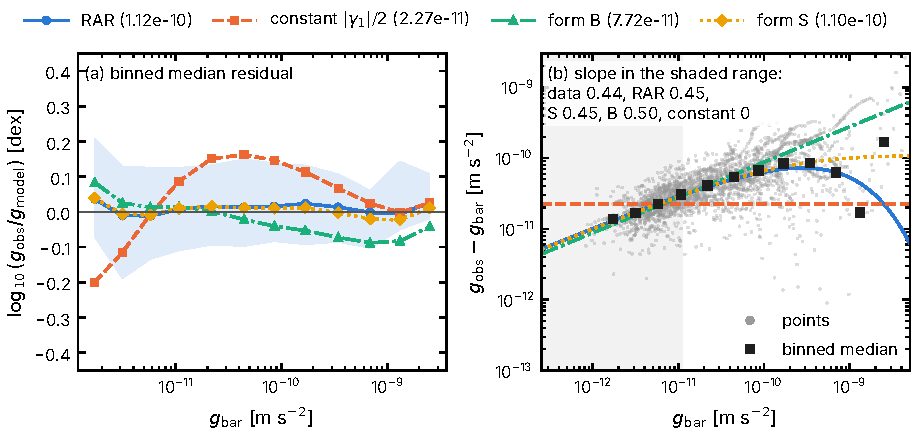
\includegraphics[width=0.9\textwidth]{remnant_forms.pdf}
\caption{(a) Binned median residual $\log(g_{\rm obs}/g_{\rm model})$ of the universal fits of Table~\ref{tab:remnant-r1} against
$g_{\rm bar}$ (band: 16--84\% of the points about the RAR). (b) The excess $g_{\rm obs}-g_{\rm bar}$: points, binned medians and the four
models. SPARC data~\cite{lelli2016} \tagS\ \chk{remnant:R1a}. Look for form B drifting low above $10^{-10}$\,m\,s$^{-2}$, the constant
missing everywhere, and form S on the RAR.}
\label{fig:remnant-forms}
\end{figure}

\paragraph{The solar system.} Both forms are pointwise laws in $g_{\rm bar}$, and the Sun's field is the cleanest $g_{\rm bar}$ there is.
Add a small radial force $f=k\,r^n$ to $GM/r^2$ and let $\epsilon=fr^2/GM$. For near-circular orbits the apsidal angle is
$\psi=\pi[3+\dd\ln F/\dd\ln r]^{-1/2}$ with $F=GM/r^2+f$, and $\dd\ln F/\dd\ln r=-2+(n+2)\epsilon+O(\epsilon^2)$, so the perihelion moves by
\begin{equation}\label{eq:precession}
\Delta\varpi=2\psi-2\pi=-\pi\,(n+2)\,\epsilon\quad\text{per orbit},
\end{equation}
which we checked by integrating orbits \chk{remnant:R1a}. Form B adds $f=\sqrt{GMa_{\rm acc}}/r$ ($n=-1$, $\epsilon=\sqrt{a_{\rm acc}/g}$),
form S adds $f\to a_{\rm acc}$ ($n=0$, $\epsilon=a_{\rm acc}/g$) for $g\gg a_{\rm acc}$. With the fitted scales, form B turns the perihelion
of Mars by $-6.0\times10^4$\,mas/yr and form S that of Saturn by $-74$\,mas/yr. The EPM2011 ephemerides allow extra precessions of
$-0.00020\pm0.00037$ and $-0.0032\pm0.0047$\,mas/yr~\cite{pitjeva2013}. Over the six planets of that analysis, form B exceeds the allowed range
by factors of $10^5$ to $1.6\times10^8$ and form S by 190 to $8\times10^4$. As written, both forms are \vd{refuted}. A surviving version needs a
rule that switches the term off at high acceleration much faster; the RAR's exponential does (its excess at Saturn is of order $10^{-331}$ of
$g$), but the accumulation picture supplies no such rule.

\subsection{Natural scales and the look-elsewhere effect}\label{sec:remnant-scales}

We fixed nine candidates for $a_{\rm acc}$ before fitting: $cH_0$, $cH_0/2\pi$, $cH_\infty$ and $cH_\infty/2\pi$ with
$H_\infty=\sqrt{\Omega_\Lambda}H_0$, $\Omega_\Lambda=0.685$, each for $H_0=67.4$~\cite{planck18} and 73\,km\,s$^{-1}$\,Mpc$^{-1}$, and $c/t_0$
with $t_0=13.8$\,Gyr. The 97 Hubble-flow distances of SPARC assume $H_0=73$~\cite{lelli2016}; rescaled to 67.4 they lower $a_{\rm acc}$ to
$1.03\times10^{-10}$ (form S) and $0.718\times10^{-10}$\,m\,s$^{-2}$ (form B). Each 67.4 candidate is compared with the rescaled data, the
others with SPARC's distances. The error on $\log a_{\rm acc}$ combines the galaxy bootstrap (0.034 dex for form S), a $\pm0.1$\,dex shift of
$\Upsilon$ (0.105) and the choice among L1, L2 and a robust loss (0.008), 0.110 dex in all; 0.131 dex for form B \chk{remnant:R1b}.

\begin{table}[t]
\centering\footnotesize
\caption{The nine candidate scales \tagS\ \chk{remnant:R1b}: fitted scale over candidate, and $\Delta$BIC of the candidate (no free
parameter) against the form's best fit on the same data. The five scales without $2\pi$ are summarised in one row (ranges).}
\label{tab:remnant-scales}
\begin{tabular}{lcccccc}
\toprule
candidate & value [m\,s$^{-2}$] & B: ratio & B: $\Delta$BIC & S: ratio & S: $\Delta$BIC & RAR $g_\dagger$: ratio\\
\midrule
$cH_0/2\pi$ ($H_0=67.4$) & $1.04\times10^{-10}$ & 0.689 & $+778$ & 0.990 & $-7.2$ & 1.009\\
$cH_0/2\pi$ ($H_0=73$) & $1.13\times10^{-10}$ & 0.684 & $+827$ & 0.973 & $-2.5$ & 0.992\\
$cH_\infty/2\pi$ ($H_0=67.4$) & $8.63\times10^{-11}$ & 0.832 & $+176$ & 1.196 & $+219$ & 1.219\\
$cH_\infty/2\pi$ ($H_0=73$) & $9.34\times10^{-11}$ & 0.826 & $+196$ & 1.176 & $+181$ & 1.198\\
$cH_0$, $cH_\infty$, $c/t_0$ (5 scales) & 5.42 to $7.09\times10^{-10}$ & 0.109--0.132 & $\geq+29979$ & 0.155--0.190 & $\geq+25096$ &
0.158--0.194\\
\bottomrule
\end{tabular}
\end{table}

The scales without $2\pi$, which a horizon argument would give (Bridge A, $cH_\infty$, among them; Section~\ref{sec:bridges}), are excluded
by $\Delta$BIC $\geq25096$ (Table~\ref{tab:remnant-scales}, Fig.~\ref{fig:remnant-scales}). Form S's $a_{\rm acc}$ lies 0.012 dex from
$cH_0/2\pi$ at $H_0=73$ and within 1\% of it when both use 67.4. This is Milgrom's coincidence $a_0\approx cH_0/2\pi$~\cite{milgrom}, which
the RAR's $g_\dagger$ shares, and it is not a test. The candidates come from a family the hypothesis does not single out, and accumulation
supplies no factor $2\pi$. They form two clusters a factor $2\pi$ apart, spanning 0.91 dex with a median spacing of 0.035 dex; four lie within
$2\sigma$ of $a_{\rm acc}$, so the data cannot choose among the $2\pi$ scales. And a scale drawn log-uniformly within $\pm1$ dex of the fit lands
as close to a candidate as observed with probability 0.10 for form S, and 0.21 for form B, whose nearest candidate is $cH_\infty/2\pi$ at
0.048 dex \chk{remnant:R1b}.

\begin{figure}[t]
\centering
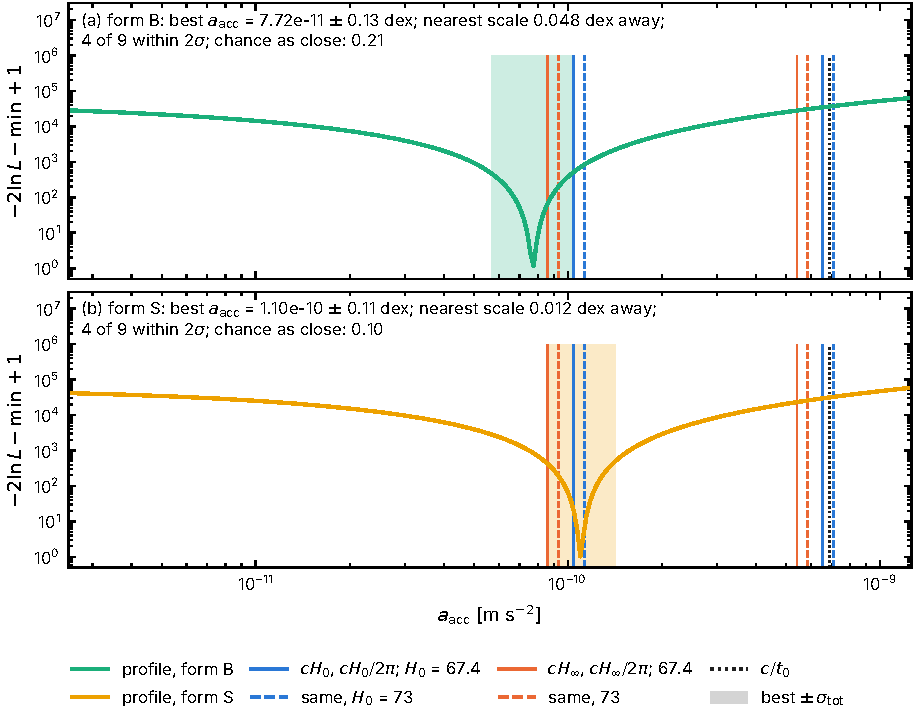
\includegraphics[width=0.9\textwidth]{remnant_scales.pdf}
\caption{$-2\ln L$ of the universal fit against $a_{\rm acc}$ for form B (a) and form S (b), with the nine candidates (solid: $H_0=67.4$,
dashed: 73, dotted: $c/t_0$) and the band $\pm\sigma_{\rm tot}$ \tagS\ \chk{remnant:R1b}. Look for the two clusters a factor $2\pi$ apart:
the minimum falls in the lower one, with four candidates inside the band.}
\label{fig:remnant-scales}
\end{figure}

\subsection{Per-galaxy scales and history}\label{sec:remnant-history}

We fitted one scale to each of the 132 galaxies with at least five points: velocity errors per point, and distance, inclination,
$\Upsilon$ ($\pm25\%$) and H\,\textsc{i} mass ($\pm10\%$) as whole-galaxy shifts, added in quadrature into an error $s_i$. The intrinsic
scatter $\tau$ of $\ell_i=\log a_i$ maximises $-\sum_i[(\ell_i-\mu)^2/(s_i^2+\tau^2)+\ln(s_i^2+\tau^2)]$.

\paragraph{Universality.} Form S gives $\tau=0.20$\,dex, as much as the RAR's per-galaxy $g_\dagger$ ($0.20$); form B gives 0.23
\chk{remnant:R1c}. Mock universes, in which the true law is the universal RAR and the data pass through the SPARC error model and the same
analysis, give $\tau=0.04$ (16--84\%: 0.00 to 0.10) for $g_\dagger$ \chk{remnant:R2}. With this error model the galaxies scatter more than a
universal law would, but equally for $g_\dagger$ and $a_{\rm acc}$: either the model misses a galaxy-level term (an $\Upsilon$ varying by more
than the assumed 0.1 dex could cause it) or neither scale is universal. Li et al.~\cite{li2018}, who marginalise each galaxy over $\Upsilon$,
distance and inclination, find no credible variation; Rodrigues et al.~\cite{rodrigues2018} conclude the opposite with a different treatment.
On universality, form S and the RAR stand or fall together.

\paragraph{History.} A universal $a_{\rm acc}$ carries no history beyond the global time. A galaxy-specific accumulation would give older,
more evolved systems a larger scale. Before computing anything we fixed five proxies and the predicted signs. $\log a_i$ should fall with
Hubble type $T$, gas fraction $1.33M_{\rm HI}/M_{\rm bar}$ and disk scale length, and rise with effective surface brightness and with the
number of orbits at the outermost measured radius in a Hubble time, $N_{\rm orb}=t_0V_{\rm out}/(2\pi R_{\rm out})$ (median 17). A fixed
variance per orbit gives $a_i\propto N_{\rm orb}$. For form B's $a_i$, the mean residual from the universal form B and the RAR's
$g_{\dagger,i}$ we computed 15 Spearman correlations and 15 partial ones at fixed $\log M_{\rm bar}$, with bootstrap intervals and the Holm
correction over all 30. A universal law fitted per galaxy with a slightly wrong shape already correlates with proxies that track where a
galaxy sits on the $g_{\rm bar}$ axis. We therefore built 500 mock universes per null model, drawing distances, inclinations, $\Upsilon$ and
gas masses from their errors and adding 0.044 dex of extra point scatter, calibrated to the data's median per-galaxy reduced $\chi^2$ of 3.01.
We tested the shift of each observed $\rho$ from the mock mean against the data's own bootstrap spread.

None of the 30 correlations survives the Holm correction (smallest adjusted $p=0.33$), and none departs from the universal-RAR baseline
(smallest adjusted $p=0.35$) \chk{remnant:R2}. Six of 15 partial correlations fall outside the mocks' 95\% bands, which understate the null
spread because the mocks lack the extra scatter found above; the shift test does not have that problem. The predicted signs hold for two of
five proxies, and the slope of $\log a_i$ on $\log N_{\rm orb}$ is $+0.12$ (95\%: $-0.17$ to $+0.46$) where a per-orbit random walk predicts
$+1$ (Fig.~\ref{fig:remnant-history}). There is no history dependence beyond the global cosmic time, and per-orbit accumulation is
\vd{refuted}.

\begin{figure}[t]
\centering
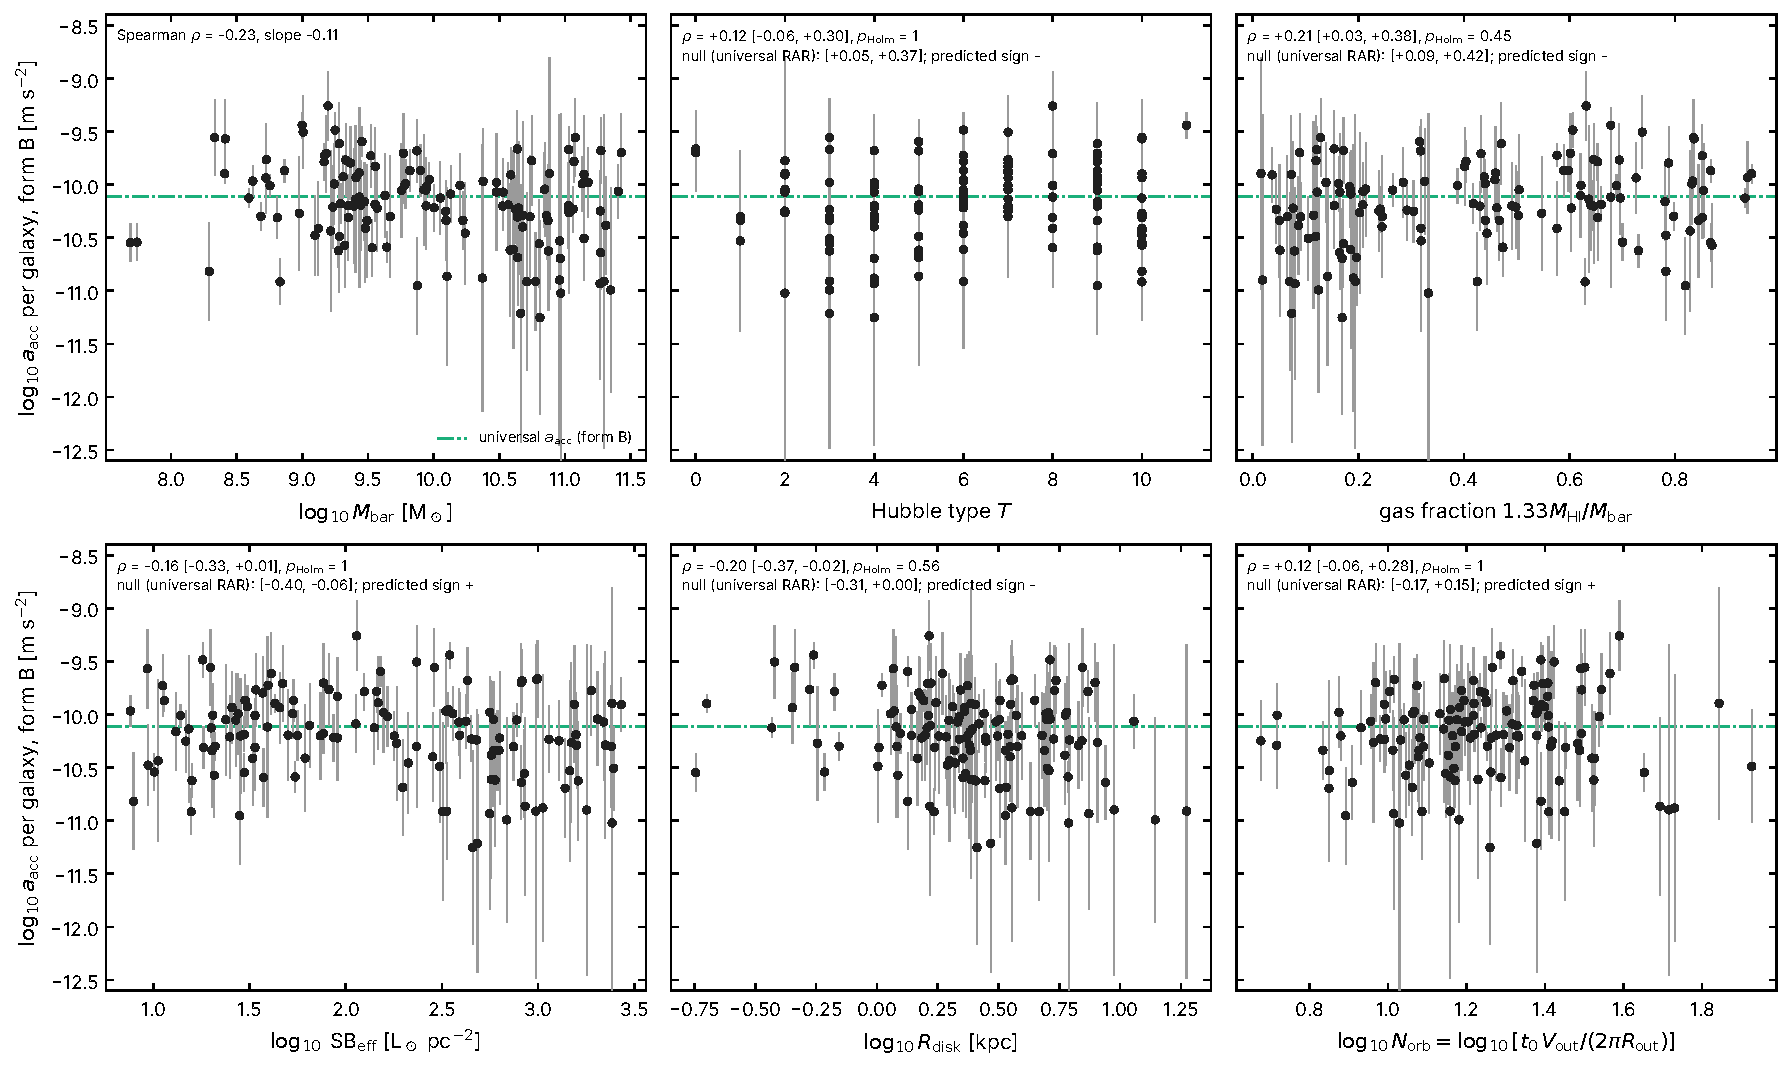
\includegraphics[width=0.8\textwidth]{remnant_history.pdf}
\caption{Per-galaxy $a_{\rm acc}$ (form B; error bars: statistical and whole-galaxy systematic) against baryonic mass and the five history
proxies, with Spearman $\rho$, its bootstrap 95\% interval, the Holm-adjusted $p$, the mock 95\% band for a universal RAR, and the predicted
sign; dash-dotted: the universal fit \tagS\ \chk{remnant:R2}. Look for the absence of the predicted trends, in particular with $N_{\rm orb}$.}
\label{fig:remnant-history}
\end{figure}

\subsection{The contained remnant: halos}\label{sec:remnant-halos}

The second route of Section~\ref{sec:darkmatter} is energy contained behind horizons at the start: primordial black holes, cold and
collisionless, which form halos as cold dark matter does. We fitted each of the 132 galaxies with $g_{\rm model}=g_{\rm bar}+GM_{\rm h}(<R)/R^2$
under L1, maximising likelihood times prior (grid, then Nelder--Mead). (i) NFW: $M_{\rm h}(<r)=M_{200}\,\mu(cr/r_{200})/\mu(c)$,
$\mu(u)=\ln(1+u)-u/(1+u)$, $M_{200}=\tfrac{4\pi}{3}200\rho_{\rm crit}r_{200}^3$ at $H_0=67.4$, with the concentration prior
$\log c_{200}=0.905-0.101\log[M_{200}/(10^{12}h^{-1}M_\odot)]$, scatter 0.11 dex~\cite{dutton2014}. (ii) Cosmological NFW: in addition, the
stellar-to-halo relation $m_\star/M_{200}=2N[(M_{200}/M_1)^{-\beta}+(M_{200}/M_1)^{\gamma}]^{-1}$ with $\log M_1=11.590$, $N=0.0351$,
$\beta=1.376$, $\gamma=0.608$ and 0.15 dex scatter~\cite{moster2013}, $m_\star=0.5L_{[3.6]}$: the halos a universe whose dark matter is all
primordial black holes must have. (iii) Burkert, cored, $\rho=\rho_0r_0^3/[(r+r_0)(r^2+r_0^2)]$, no prior. The per-galaxy BIC counts $k=2$ for
a halo, 1 for a free scale and 0 for a universal law.

\begin{table}[t]
\centering\footnotesize
\caption{Halos against universal laws, 132 galaxies, 2652 points \tagS\ \chk{remnant:R3}. $\Delta$BIC: summed over galaxies, relative to
the universal RAR. Last column: galaxies whose own BIC beats the universal RAR's.}
\label{tab:remnant-halos}
\begin{tabular}{lrrrr}
\toprule
model & parameters & $-2\ln L$ & $\Delta$BIC & better than RAR\\
\midrule
RAR, universal $g_\dagger$ & 1 & $-2478.0$ & 0 & --\\
form S, universal $a_{\rm acc}$ & 1 & $-2482.6$ & $-4.6$ & 64\\
form B, universal $a_{\rm acc}$ & 1 & $-2259.9$ & $+218$ & 54\\
RAR, one $g_\dagger$ per galaxy & 132 & $-5393.8$ & $-1883$ & 85\\
NFW, concentration prior & 264 & $-5911.6$ & $-1360$ & 88\\
NFW, concentration and stellar-to-halo prior & 264 & $-5659.1$ & $-1108$ & 82\\
Burkert & 264 & $-6331.5$ & $-1780$ & 98\\
\bottomrule
\end{tabular}
\end{table}

Every per-galaxy model beats every universal law in total BIC (Table~\ref{tab:remnant-halos}) \tagS. This is largely because L1 treats a
galaxy's common distance, inclination and $\Upsilon$ errors as independent per point, so any per-galaxy parameter gains by absorbing them:
one free RAR scale per galaxy reaches $-1883$. Against that yardstick NFW halos are worse by $\Delta$BIC $+523$, Burkert halos by $+103$ and
cosmological NFW halos by $+775$; cored halos beat cuspy ones by $-420$ at equal parameter count, the known cusp-core issue. The NFW halos
have $\log M_{200}=11.47$ (16--84\%: 10.76 to 12.18), about 24 times the baryonic mass. They accommodate the RAR's one-parameter regularity
with two parameters per galaxy; they do not predict it.

\subsection{Halos and a universal stochastic term together}\label{sec:remnant-joint}

The cohesive whole would be baryons, a halo per galaxy and one universal term, $S=A$ or $S=\sqrt{g_{\rm bar}A}$. At each of 66 amplitudes
from $10^{-16}$ to $10^{-9.5}$\,m\,s$^{-2}$ we refitted every halo and summed the profile
$T(A)=\sum_i\min_{\theta_i}[-2\ln L_i(\theta_i,A)-2\ln\pi(\theta_i)]$ ($\pi$: halo prior). The one-sided 95\% bound is where $T$ rises by 2.71
above its minimum; adding the term costs $\Delta\mathrm{BIC}=T(\hat A)-T(0)+\ln N$.

\begin{table}[t]
\centering\footnotesize
\caption{A universal term added to halos \tagS\ \chk{remnant:R4}. Bound: one-sided 95\%, with its galaxy-bootstrap 84th percentile in
brackets. Share: median fraction of the dark acceleration $g_{\rm obs}-g_{\rm bar}$ at each galaxy's outermost point that the term supplies at
the bootstrap bound. Alone, the square-root term needs $7.7\times10^{-11}$ and the constant $2.3\times10^{-11}$\,m\,s$^{-2}$.}
\label{tab:remnant-joint}
\begin{tabular}{llrrrr}
\toprule
halos & term & best $A$ [m\,s$^{-2}$] & $\Delta$BIC & 95\% bound [m\,s$^{-2}$] & share\\
\midrule
NFW & $\sqrt{g_{\rm bar}A}$ & 0 & $+7.9$ & $2.1\times10^{-15}$ ($6.5\times10^{-15}$) & 1.0\%\\
NFW, cosmological & $\sqrt{g_{\rm bar}A}$ & 0 & $+7.9$ & $2.3\times10^{-15}$ ($3.0\times10^{-14}$) & 2.1\%\\
Burkert & $\sqrt{g_{\rm bar}A}$ & 0 & $+7.9$ & $1.3\times10^{-14}$ ($1.4\times10^{-13}$) & 4.5\%\\
NFW & constant & 0 & $+7.9$ & $8.4\times10^{-13}$ ($3.5\times10^{-12}$) & 16\%\\
NFW, cosmological & constant & $6.6\times10^{-13}$ & $+3.5$ & $1.2\times10^{-12}$ ($1.9\times10^{-12}$) & 8.5\%\\
Burkert & constant & $4.2\times10^{-12}$ & $-50.1$ & $5.1\times10^{-12}$ ($6.7\times10^{-12}$) & 31\%\\
\bottomrule
\end{tabular}
\end{table}

With NFW halos, with or without the cosmological prior, the best square-root amplitude is zero (in 87 to 97\% of the galaxy resamples), and
the profile rises roughly as $\sqrt A$: the refitted halos cannot absorb the term, so it costs at first order (Table~\ref{tab:remnant-joint},
Fig.~\ref{fig:remnant-halos}) \tagS. With cosmological halos its bound at the bootstrap 84th percentile, $3.0\times10^{-14}$, is about 2600
times below what form B needs alone; a constant is bounded at 4 to 5\% of the value that replaces the halos. Only cored halos prefer a small
constant ($4.2\times10^{-12}$, $\Delta$BIC $-50$); since NFW halos do not, we read it as a correction to the halo's outer shape, not a
universal term.

\paragraph{The consistency requirement.} The acoustic peaks fix $\Omega_ch^2=0.120\pm0.001$ of collisionless matter at
$z\approx1100$~\cite{planck18}. If that is the contained remnant, halos of cosmological mass exist, and a stochastic term must not count their
dark acceleration a second time. The room left, with cosmological halos: a median 2.1\% of the dark acceleration at the outermost measured
radius for the square-root term, 8.5\% for the constant \chk{remnant:R4}.

\begin{figure}[t]
\centering
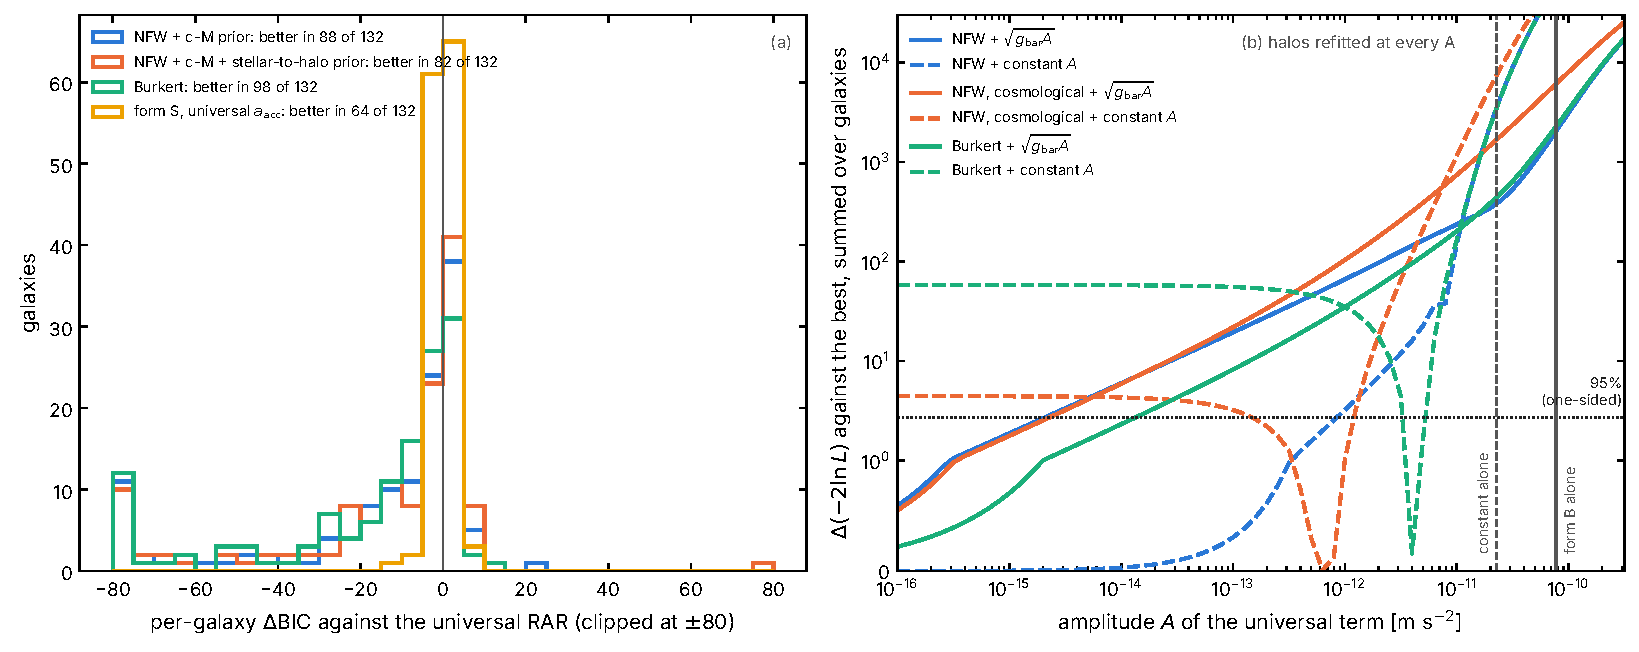
\includegraphics[width=0.9\textwidth]{remnant_halos.pdf}
\caption{(a) Per-galaxy $\Delta$BIC of three halo models and of the universal form S against the universal RAR (negative: better; clipped at
$\pm80$). (b) $\Delta(-2\ln L)$ summed over 132 galaxies, every halo refitted, against the amplitude of a universal term (solid:
$\sqrt{g_{\rm bar}A}$, dashed: constant), with the one-sided 95\% level and the values each term needs alone \tagS\
\chk{remnant:R3,R4}. Look for the square-root curves leaving zero at once, orders of magnitude below the value the term needs to matter.}
\label{fig:remnant-halos}
\end{figure}

\subsection{Cosmic time}\label{sec:remnant-time}

We compare four laws, fixed in advance: $a_{\rm acc}$ constant; $\propto H(z)=H_0[\Omega_m(1+z)^3+\Omega_\Lambda]^{1/2}$; $\propto1/t$; and
$\propto t$, the random-walk accumulation. In flat $\Lambda$CDM with $\Omega_m=0.315$~\cite{planck18},
$t(z)=\tfrac{2}{3H_0\sqrt{\Omega_\Lambda}}\,\mathrm{arsinh}[\sqrt{\Omega_\Lambda/\Omega_m}(1+z)^{-3/2}]$. In the deep regime $V^4=GMa_{\rm acc}$, so
at fixed rotation speed $\Delta\log M_{\rm bar}(z)=-\log[a_{\rm acc}(z)/a_{\rm acc}(0)]$. Massive disks at high redshift are not deep: their
half-light radii sit at 3 to 11 $a_0$~\cite{milgrom2017}. We therefore also give the shift for a RAR-shaped law at fixed $V$ and $R$ with
$g_{\rm obs}=3g_\dagger$, where any change of scale is diluted (Table~\ref{tab:remnant-time}).

\begin{table}[t]
\centering\footnotesize
\caption{Evolution laws \tagS\ \chk{remnant:R5}: $a(z)/a(0)$, and $\Delta\log M_{\rm bar}$ [dex] at fixed rotation speed in the deep regime
and at $g_{\rm obs}=3g_\dagger$.}
\label{tab:remnant-time}
\begin{tabular}{lcccccc}
\toprule
& \multicolumn{2}{c}{$a(z)/a(0)$} & \multicolumn{2}{c}{deep} & \multicolumn{2}{c}{$3g_\dagger$}\\
\cmidrule(lr){2-3}\cmidrule(lr){4-5}\cmidrule(lr){6-7}
law & $z=1$ & $z=2$ & $z=0.9$ & $z=2.3$ & $z=0.9$ & $z=2.3$\\
\midrule
constant & 1.00 & 1.00 & 0 & 0 & 0 & 0\\
$\propto H(z)$ & 1.79 & 3.03 & $-0.23$ & $-0.54$ & $-0.07$ & $-0.22$\\
$\propto 1/t$ & 2.36 & 4.21 & $-0.34$ & $-0.69$ & $-0.12$ & $-0.31$\\
$\propto t$ (accumulation) & 0.42 & 0.24 & $+0.34$ & $+0.69$ & $+0.07$ & $+0.10$\\
\bottomrule
\end{tabular}
\end{table}

\paragraph{Measurements.} \"Ubler et al.~\cite{ubler2017} fit the baryonic Tully--Fisher relation of KMOS$^{\rm 3D}$ disks with the local
slope 3.75 and find zero-point offsets of $-0.44\pm0.04$\,dex at $z\approx0.9$ (65 galaxies) and $-0.27\pm0.05$ at $z\approx2.3$ (46),
statistical errors only; without their pressure-support correction, $-0.33$ and $-0.09$. Their baryonic masses carry about 0.15 dex each,
with gas from scaling relations. Read as a change of scale they imply $a(z)/a(0)=2.8$ (deep) to 7.6 ($3g_\dagger$) at $z\approx0.9$ and 1.9
to 4.2 at $z\approx2.3$ \chk{remnant:R5}. MUSE-DARK III~\cite{ciocan2026} fits the RAR of 79 galaxies at $0.33<z<1.44$:
$a_0(z\approx1)=2.38^{+0.12}_{-0.10}\times10^{-10}$\,m\,s$^{-2}$, $1.98\pm0.44$ times the local 1.2, with $g_{\rm obs}$ and $g_{\rm bar}$ from one
model. Six rotation curves at $z\approx0.9$--2.4 ``all but exclude'' a MOND constant of about $4a_0$ at $z\approx2$~\cite{milgrom2017}. The
dark-matter fractions of 100 massive disks, $0.38\pm0.23$ at $z=0.6$--1.2 and $0.27\pm0.18$ at $z=1.2$--2.5 (median and
scatter)~\cite{nestorshachar2023}, would need each galaxy's $g_{\rm bar}$ and are not used.

\paragraph{Comparison.} Accumulation predicts a smaller scale in the past, hence more baryons at fixed speed; every measurement points the
other way (Fig.~\ref{fig:remnant-redshift}). At $z=1$, MUSE-DARK's $2.0\pm0.4$ lies between the $H(z)$ and $1/t$ laws; at $z=2$ the $1/t$
law reaches the $4a_0$ that Milgrom finds all but excluded. The \"Ubler offsets have the sign of a larger past scale, but in the deep reading
the one at $z\approx0.9$ is larger and the one at $z\approx2.3$ smaller than either falling law predicts, and no monotonic law fits both. The
systematics (gas masses, pressure support, model-dependent $g_{\rm bar}$) are as large as the effect, and $\Lambda$CDM galaxy evolution makes
such offsets too, so this is not a clean test; read literally, the data disfavour accumulation. The two time arrows also disagree in
principle: an accumulated scale grows with time, while $cH$ and $c/t$ fall, so an $a_{\rm acc}$ that accumulates and equals $cH_0/2\pi$ today
does so by a coincidence of the present epoch.

\begin{figure}[t]
\centering
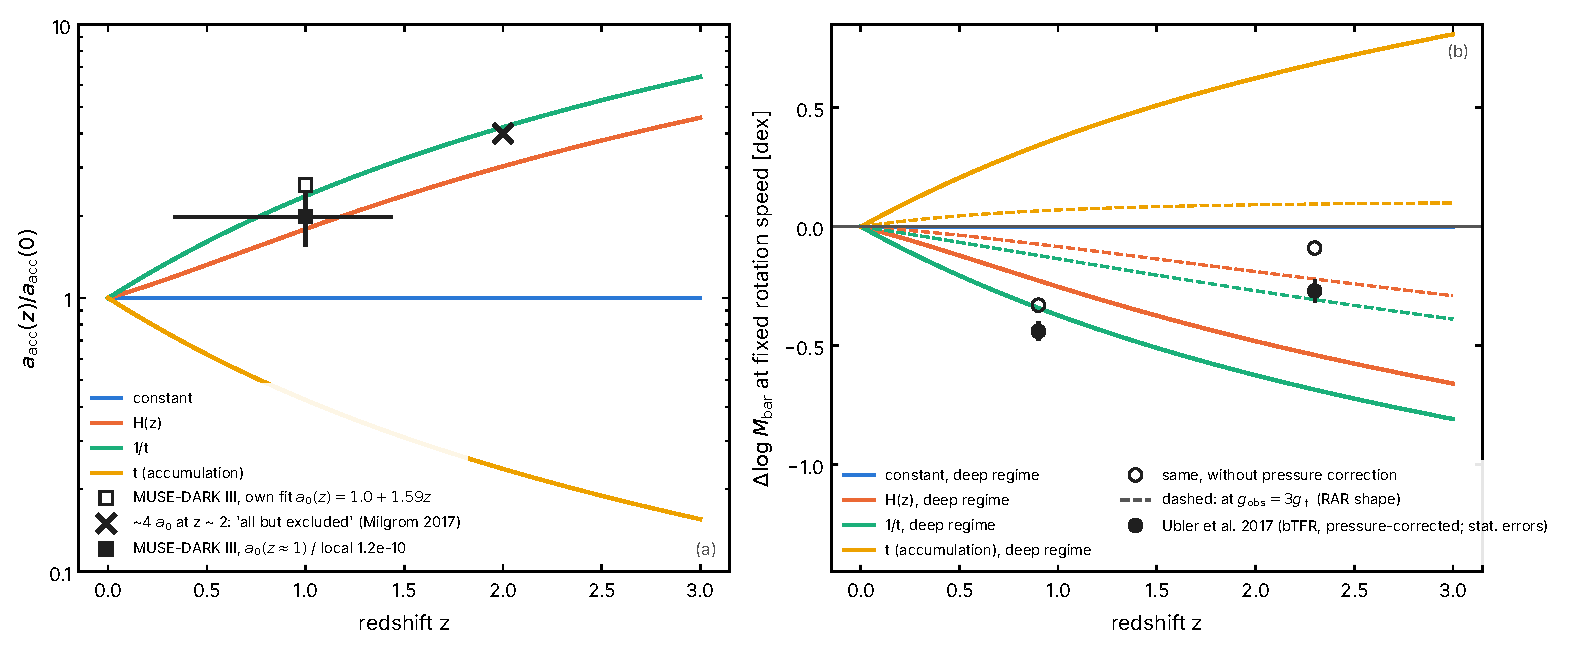
\includegraphics[width=0.9\textwidth]{remnant_redshift.pdf}
\caption{(a) The four laws for $a_{\rm acc}(z)/a_{\rm acc}(0)$, MUSE-DARK III at $z\approx1$ (filled: against the local 1.2; open: their
linear fit) and the value Milgrom finds all but excluded at $z\approx2$. (b) $\Delta\log M_{\rm bar}$ at fixed rotation speed, deep (solid)
and at $3g_\dagger$ (dashed), with the \"Ubler et al.\ offsets (filled: pressure-corrected, statistical errors; open: uncorrected) \tagS\
\chk{remnant:R5}. Look for the sign: accumulation lies above zero, every measurement below.}
\label{fig:remnant-redshift}
\end{figure}

\subsection{What cannot be fitted}\label{sec:remnant-cannot}

The stochastic remnant exists only as the Newtonian limit of a static, spherically symmetric calculation~\cite{oppenheimrusso}. The acoustic
peaks need $\Omega_ch^2=0.120$ of pressureless matter at $z\approx1100$~\cite{planck18} and hence a cosmological perturbation theory of the
remnant; there is none, and lensing, which needs the metric, is left open by its authors: both \vd{untested}. MOND-like laws reduce the mass
discrepancy of clusters three- to four-fold but do not remove it~\cite{sanders2003}; forms B and S inherit that residual (no cluster test was
run). In the merging cluster 1E0657$-$558 the lensing mass follows the galaxies, offset from the X-ray gas at $8\sigma$~\cite{clowe}: a term
set by the local baryonic field follows the gas, collisionless halos follow the galaxies. The contained remnant is cold dark matter and covers
all four as $\Lambda$CDM does (\vd{holds as a reading}).

\paragraph{Choices made after seeing the data.} (1) The amplitude grid of Section~\ref{sec:remnant-joint} first started at
$10^{-13}$\,m\,s$^{-2}$; the first run put the square-root bound below it, and $\sqrt{10^{-12}\cdot10^{-13}}$ is 30\% of the lowest
$g_{\rm bar}$, so the grid now starts at $10^{-16}$ and the fitter's consistency check uses $10^{-30}$. (2) Two checks failed on the first run
because the checks were wrong (a logarithm base, an angle unwrapping); they were fixed and no tolerance was loosened. (3) The mocks were raised
from 200 to 500 per null model after a test run. (4) The mocks' extra point scatter is calibrated on the data. (5) One free RAR scale per
galaxy was chosen as the halos' yardstick after seeing that every per-galaxy model beats every universal one. (6) Reading the Burkert constant
as a halo-shape correction is an interpretation made after seeing it. (7) The shift test and the mock calibration of $\tau$ were added after
test runs with 4 to 20 mocks, whose bands looked narrower than the bootstrap intervals; bands, tests and calibration are all reported.

\paragraph{Caveats.} $\Upsilon$ is fixed at 0.5 and 0.7 throughout, with $m_\star=0.5L_{[3.6]}$ (bulge light at the disk value) in the
stellar-to-halo prior; a free $\Upsilon$ with a prior would improve the halo fits and the universal laws alike. The stellar-to-halo relation
was derived for a WMAP7 cosmology, and we did not check how well it is constrained at SPARC's lowest stellar masses. The halos are not
adiabatically contracted. The high-redshift comparison uses published summary numbers whose systematics match the predicted effects, for
massive disks selected differently from SPARC.

All numbers in this section come from \texttt{docs/simulation/remnant\_history.py} (39 of 39 checks, about two and a half minutes on one
core).

\paragraph{Verdict.} An accumulated stochastic remnant of the self-consistent form fits the rotation curves as well as the radial acceleration
relation, but it is MOND's simple interpolating function: its scale matches $cH_0/2\pi$ only as Milgrom's $a_0$ always has, it is
\vd{refuted} in the solar system as a pointwise law, it carries no galaxy-specific history, and the high-redshift data favour a scale that was
larger in the past, not one that accumulates. The contained remnant, primordial black holes as cold dark matter, covers the microwave
background, lensing and the merging cluster and fits the rotation curves with two parameters per galaxy (\vd{live}); once its halos are
present, the stochastic term is bounded to a few per cent of the dark acceleration. The two remnants compete rather than combine, and the
consistent reading of Hypothesis~H7 is primordial black holes as the cold dark matter, with a stochastic term too small to matter in galaxies.
